\documentclass[a4paper, 12pt]{article}%тип документа

%отступы
\usepackage[left=2cm,right=2cm,top=2cm,bottom=3cm,bindingoffset=0cm]{geometry}

%Русский язык
\usepackage[T2A]{fontenc} %кодировка
\usepackage[utf8]{inputenc} %кодировка исходного кода
\usepackage[english,russian]{babel} %локализация и переносы

%Вставка картинок
\usepackage{wrapfig}
\usepackage{graphicx}
\graphicspath{{pictures/}}
\DeclareGraphicsExtensions{.pdf,.png,.jpg}

%оглавление
\usepackage{titlesec}
\titlespacing{\chapter}{0pt}{-30pt}{12pt}
\titlespacing{\section}{\parindent}{5mm}{5mm}
\titlespacing{\subsection}{\parindent}{5mm}{5mm}
\usepackage{setspace}

%Графики
\usepackage{multirow}
\usepackage{pgfplots}
\pgfplotsset{compat=1.9}

%Математика
\usepackage{amsmath, amsfonts, amssymb, amsthm, mathtools}

%Стиль страницы
\usepackage{fancyhdr}
\pagestyle{fancy}

\begin{document}

\begin{titlepage}

\begin{center}
%\vspace*{1cm}
\large\textbf{Московский Физико-Технический Институт}\\
\large\textbf{(государственный университет)}
\vfill
\line(1,0){430}\\[1mm]
\huge\textbf{Работа 5.2.1}\\
\line(1,0){430}\\[1mm]
\vfill
\large Сибгатуллин Булат, ФРКТ\\
\end{center}

\end{titlepage}
\fancyhead[L] {Работа 5.2.1}
\noindent \textbf{Цель работы:} \\
\indent Методом электронного возбуждения измерить энергию первого уровня атома гелия в динамическом и статическом режимах\\

\section*{Описание работы}
Опыт Франка-Герца подтверждает существование дискретных уровней энергии атомов. Разреженный одноатомный газ заполняет трёхэлектродную лампу. Электроны, испускаемые разогретым катодом, ускоряются в постоянном электрическом поле, созданном между катодом и сетчатым анодом лампы. Передвигаясь от катода к аноду, электроны сталкиваются с атомами гелия.
\begin{itemize}
    \item энергия электрона недостаточна, чтобы возбудить/ионизировать атом -> \textit{упругое столкновение}, электрон не теряет энергию
    \item при большой разности потенциалов энергия электрона достаточна для возбуждения атомов -> \textit{неупругое столкновение}, кинетическая энергия передаётся одному из атомных электронов, в результате чего происходит:
    \begin{itemize}
        \item \textbf{возбуждение} - переход одного из атомных электронов на свободный энергетический уровень
        \item \textbf{ионизация} - отрыв электрона от атома 
    \end{itemize}
\end{itemize}

\begin{figure}[h]
\begin{center}
\begin{minipage}[h]{0.45\linewidth}
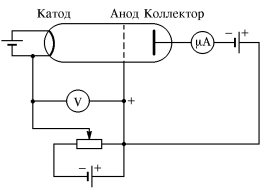
\includegraphics[width=1\linewidth]{images/fig1.PNG}
\caption{Схема опыта Франка и Герца} %% подпись к рисунку
\label{ris:experimoriginal} %% метка рисунка для ссылки на него
\end{minipage}
\hfill 
\begin{minipage}[h]{0.45\linewidth}
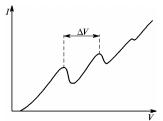
\includegraphics[width=1\linewidth]{images/fig2.PNG}
\caption{Схематический вид зависимости тока коллектора от напряжения на аноде}
\label{ris:experimcoded}
\end{minipage}
\end{center}
\end{figure}

Объясним вид зависимости тока коллектора (измеряется микроамперметром) от напряжения на аноде. При увеличении потенциала анода ток в лампе сначала растёт (зависимость, подобная ВАХ вакуумного диода). Когда энергия электронов становится достаточной для возбуждения атомов, ток коллектора резко уменьшается. Это происходит потому, что при неупругих соударениях с атомами электроны теряют свою энергию и не могут преодолеть задерживающее напряжение (около 1 В) между анодом и коллектором. При дальнейшем увеличении потенциала ток коллектора вновь возрастает: электроны, испытавшие неупругие соударения, при дальнейшем движении к аноду успевают набрать энергию, достаточную для преодоления задерживающего потенциала. Следующее замедление роста тока происходит в момент, когда часть электронов неупруго сталкивается с атомами два раза. Таким образом, на кривой зависимости тока коллектора от напряжения анода имеется ряд максимумов и минимумов, отстоящих друг от друга на равные расстояния, равные энергии первого возбуждённого состояния.

\section{Экспериментальная установка}

\begin{figure}[h]
    \centering
    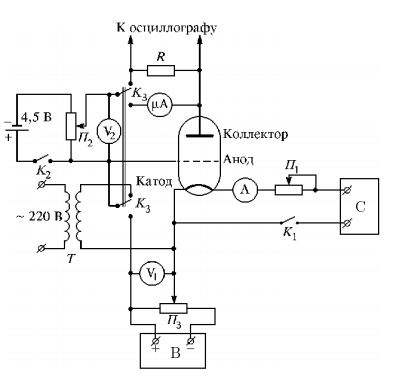
\includegraphics[width=12cm]{images/fig3.PNG}
    \caption{Схема экспериментальной установки}
    \label{fig:vac}
\end{figure}

На рис.3 обозначены:
\begin{itemize}
    \item А - амперметр
    \item Б7-4 - стабилизированный источник питания (подаёт напряжение накала)
    \item $K_1$ - тумблер для включения в цепь источника Б7-4
    \item Б5-10 - выпрямитель (подаёт на анод ускоряющее напряжение)
    \item $Pi_3$ - потенциометр, регулирующий величину ускоряющего напряжения
    \item $V_1$ - вольтметр, измеряющий величину ускоряющего напряжения
    \item 4,5 В - батарея КБСЛ - источник задерживающего потенциала
    \item $Pi_2$ - потенциометр, регулирующий величину задерживающего потенциала
    \item $V_2$ - вольтметр, измеряющий величину задерживающего потенциала
    \item $\mu A$ - микроамперметр - регистрирует ток в цепи коллектора
    \item $K_3$ - ключ, переключающий схему из статического режима в динамический
    \item Т - понижающий трансформатор - подаёт ускоряющий потенциал при динамическом режиме
    \item - нагрузочный резистор
\end{itemize}

\section{Выполнение работы}

\subsection{Динамический метод}

\begin{enumerate}

\item Подготовим приборы к работе, поставим переключатель режима в положение "Динамич."
   
\item Добьёмся с помощью регуляторов на осциллографе чёткой картины на экране

\item При максимальном ускоряющем напряжении измерим на экране расстояние между максимумами и между минимумами осциллограммы. Измерения проведём при трёх значениях задерживающего напряжения: 4, 6 и 8 В. Результаты измерений занесём в таблицу 1. Фотографии полученных осциллограмм приведём на рисунках 4-6.

\begin{center}
\begin{tabular}{ |p{3.5cm}||p{1cm}|p{1cm}|p{1cm}|p{1cm}|p{2.5cm}|p{1cm}|p{1cm}|}
 \hline
Задерж. напряжение & $V_{max_1}$ & $V_{max_2}$ & $V_{min_1}$ & $V_{min_2}$ & Погрешность & $\triangle V_{max}$ & $\triangle V_{min}$\\
 \hline
 4 В & -3 В & 11 В & 0 В & 18 В & 1 В & 14 В & 18 В\\
\hline
 6 В & -6 В & 8 В & -3 В & 17 В & 1 В & 14 В & 20 В\\
\hline
 8 В & -9 В & 5 В & -5 В & 15 В & 1 В & 14 В & 20 В\\
\hline

\end{tabular}
\end{center}

\begin{figure}[h]
\begin{center}
\begin{minipage}[h]{0.45\linewidth}
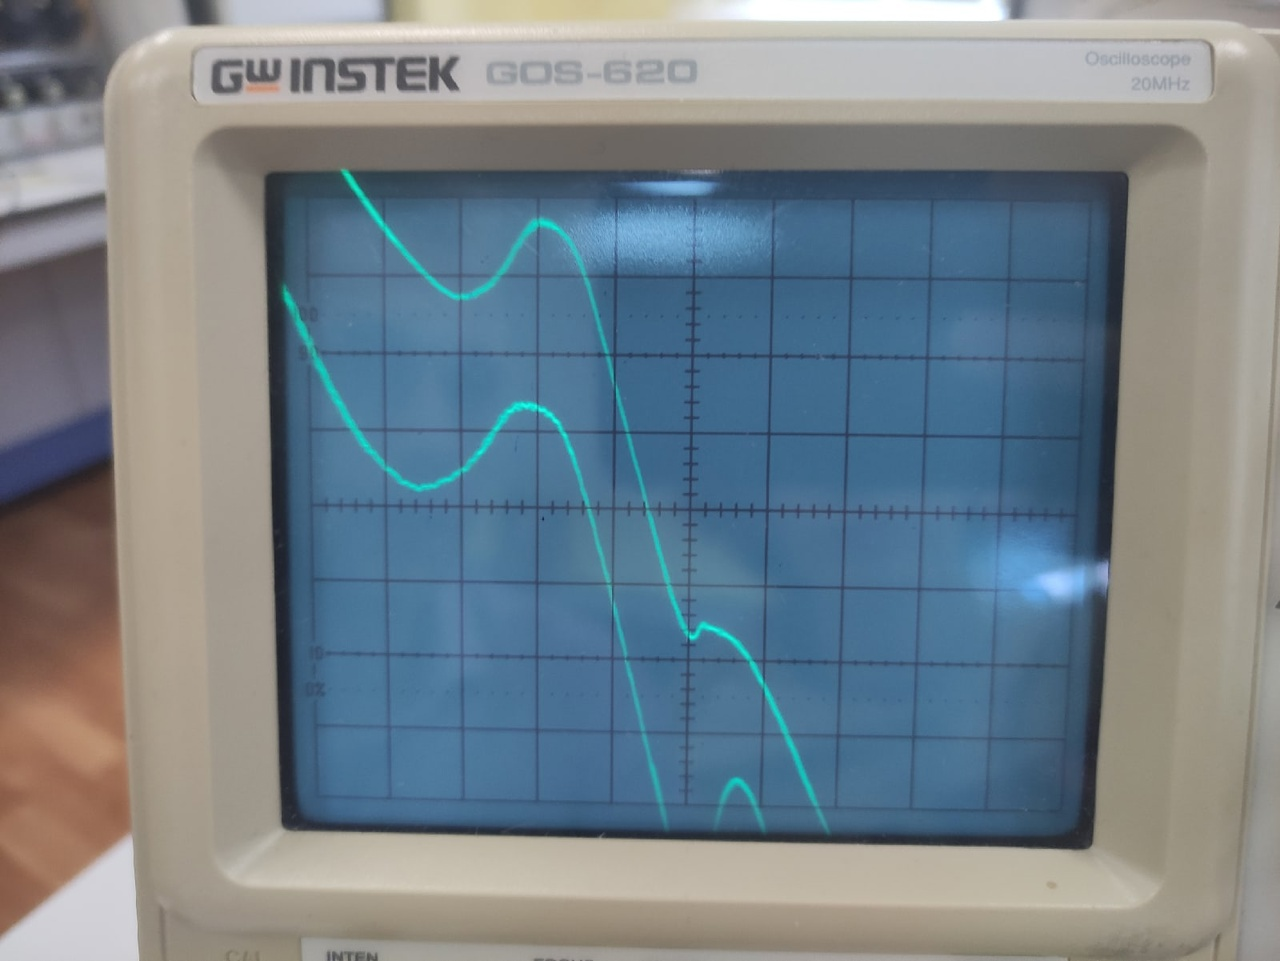
\includegraphics[width=1\linewidth]{images/1.jpg}
\caption{Осциллограмма при задерживающем напряжении 4 В} %% подпись к рисунку
\label{ris:experimoriginal} %% метка рисунка для ссылки на него
\end{minipage}
\hfill 
\begin{minipage}[h]{0.45\linewidth}
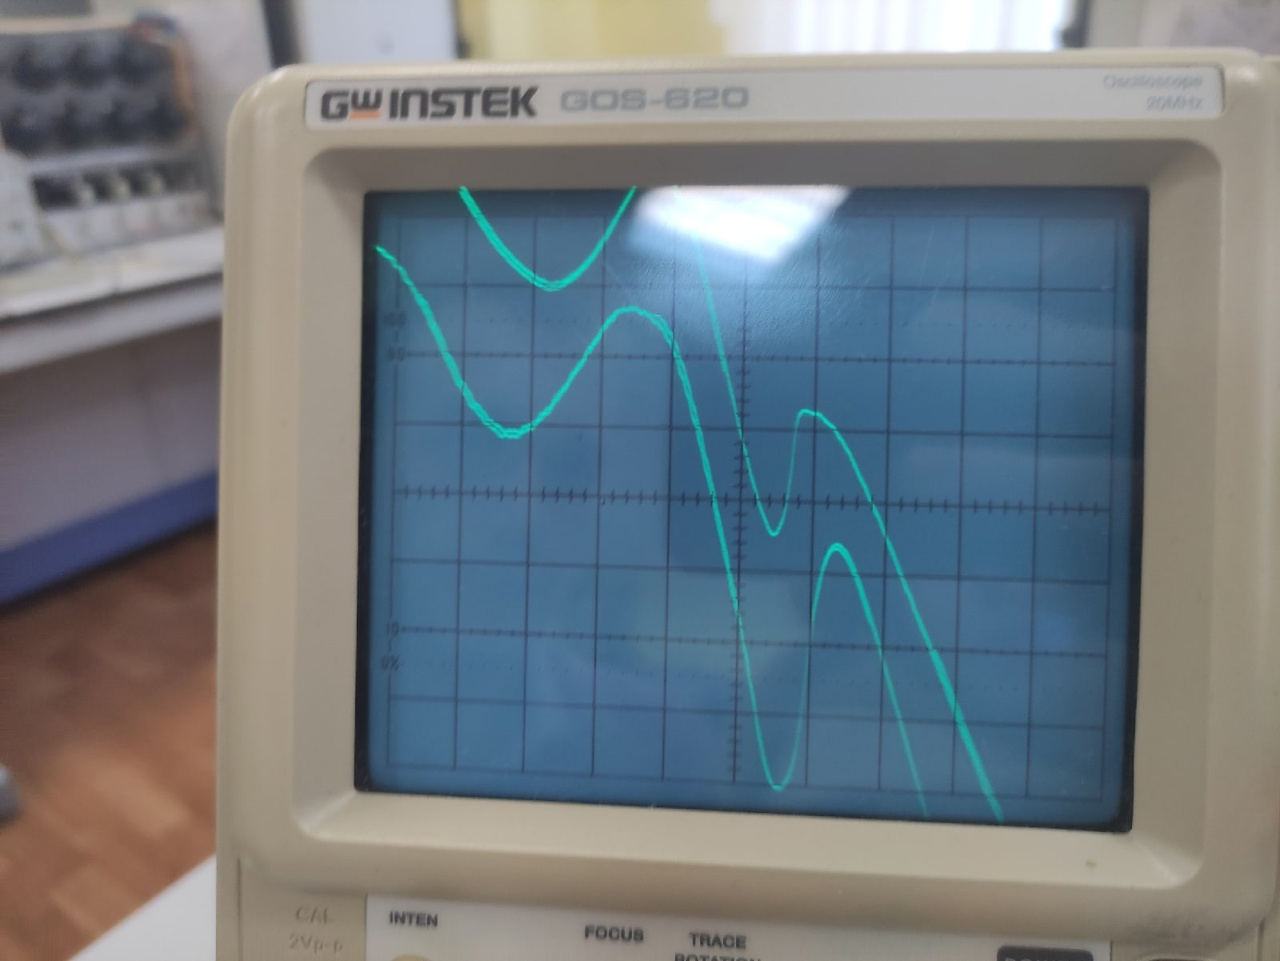
\includegraphics[width=1\linewidth]{images/2.jpg}
\caption{Осциллограмма при задерживающем напряжении 6 В}
\label{ris:experimcoded}
\end{minipage}
\hfill 
\begin{minipage}[h]{0.45\linewidth}
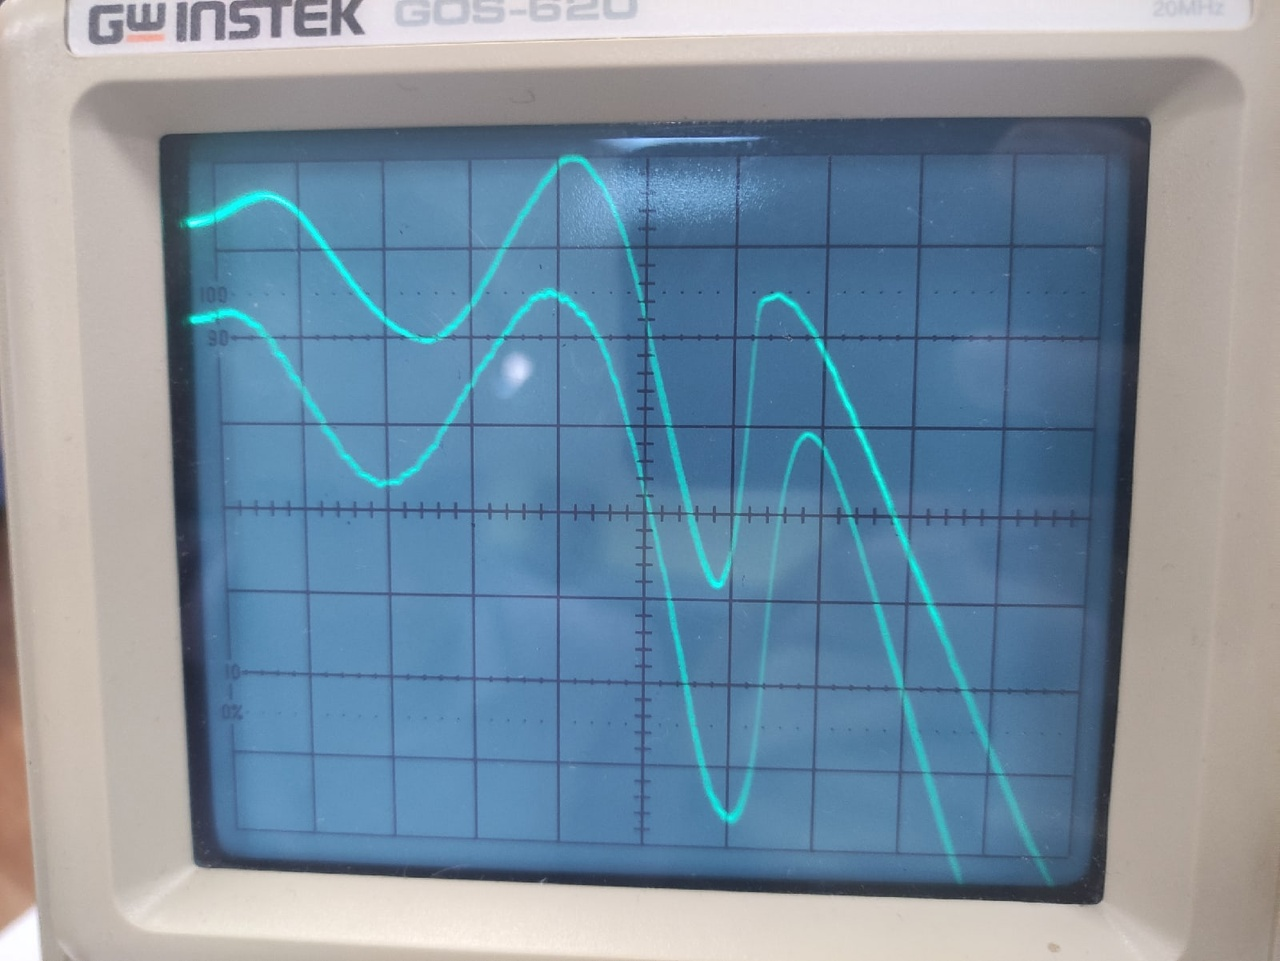
\includegraphics[width=1\linewidth]{images/3.jpg}
\caption{Осциллограмма при задерживающем напряжении 8 В}
\label{ris:experimcoded}
\end{minipage}
\end{center}
\end{figure}

\item Определим значение энергии первого возбуждённого состояния атома гелия. 
\begin{center}
    $\overline{V_{max}} = 14$ В \hspace{1cm} $\overline{V_{min}} = 19.3$ В
\end{center}
Погрешности определения средних значений определим, используя формулу
\begin{center}
    $\sigma^2_{V_1} = \sigma^2_{V_4} + \sigma^2_{V_6} + \sigma^2_{V_8}$ - погрешность прибора \\
    $\sigma_{V_2} = \sqrt{\frac{1}{6}\sum (V_i - \overline{V})^2}$ -  погрешность среднего значения \\
    $\sigma_{V_1} = 1.7$ В \hspace{1cm} $\sigma_{V_{max_2}} = 0$ В  \hspace{1cm} $\sigma_{V_{min_2}} = 0.5$ В
\end{center}

В итоге получаем:
\begin{center}
    $\overline{V_{max}} = 14.0 \pm 1.7$ В \hspace{1cm} $\overline{V_{min}} = 19.3 \pm 1.8	$ В
\end{center}


Среднее значение первого возбуждённого состояния атома гелия по результатам эксперимента:
\begin{center}
    $V_{exp} = 16.7 \pm 2.5$ эВ (относительная погрешность составляет 14\%)
\end{center}
При этом табличное значение данной величины составляет
\begin{center}
    $V_{th} = 21.6$ эВ
\end{center}
С учётом погрешности, экспериментальные данные немного отличаются от теоретических. Это может быть обусловлено низкой точностью измерений, так как на сетке осциллографа плохо видно, на каком делении лежит максимум или минимум графика. Также максимум и мунимумы в таком масштабе выглядят пологими, следовательно мы не можем точно определить, где именно  находится максимум или минимум. Из-за этого мы получаем погрешность измерений, которую становится тяжело учесть. В качестве решения этой проблемы мы можем увеличить погрешность измерения с 1 до 2 вольт, но в таком случае и погрешность итогового значения увеличится в 2 раза, что приведет к очень низкой точности измерения, да и увеличение погрешности только из-за того, что значение не сошлось с табличным, может наоборот испортить значения измерений.

\end{enumerate}

\subsection{Статический метод}

\begin{enumerate}
    \item Переведём переключатель режима в положение <<Статич.>>, установим максимальный ток накала
    \item Снимем зависимость коллекторного тока от анодного напряжения $I_k = f(V_a)$ для значений задерживающего напряжения 4, 6 и 8 В. Результаты измерений занесём в таблицы 2-4 (рисунки 7-9).
    
    \begin{figure}[h]
    \centering
    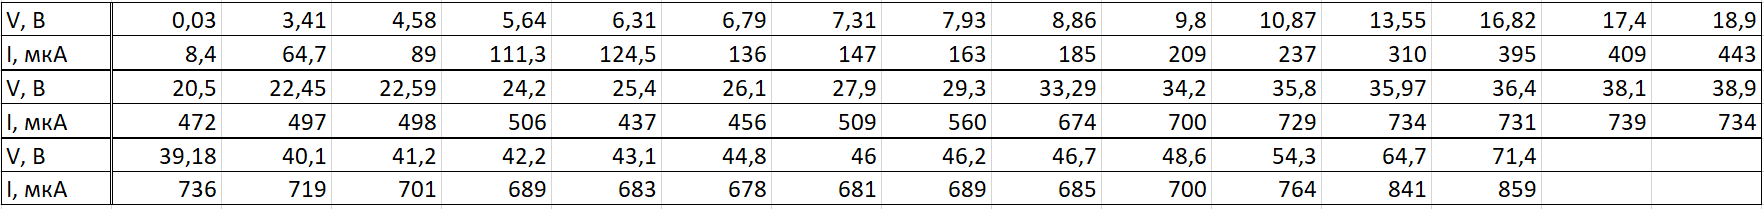
\includegraphics[width=0.9\linewidth]{images/4_V.PNG}
    \caption{Значения коллекторного тока и анодного напряжения, задерживающее напряжение 4 В}
    \label{fig:vac}
\end{figure}

\begin{figure}[h]
    \centering
    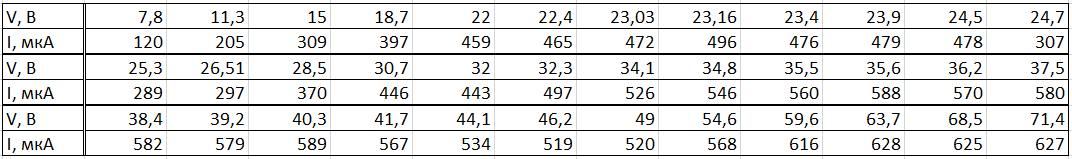
\includegraphics[width=0.9\linewidth]{images/6_V.PNG}
    \caption{Значения коллекторного тока и анодного напряжения, задерживающее напряжение 6 В}
    \label{fig:vac}
\end{figure}

\begin{figure}[h]
    \centering
    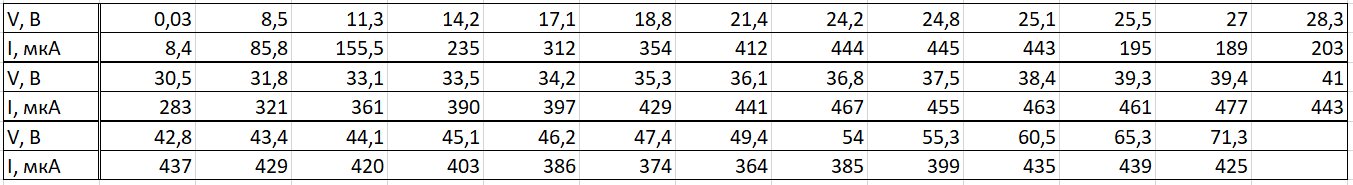
\includegraphics[width=0.9\linewidth]{images/8_V.PNG}
    \caption{Значения коллекторного тока и анодного напряжения, задерживающее напряжение 8 В}
    \label{fig:vac}
\end{figure}

\item Перенесем полученные значения на график:

\begin{figure}[h]
\begin{center}
\begin{minipage}[h]{0.45\linewidth}
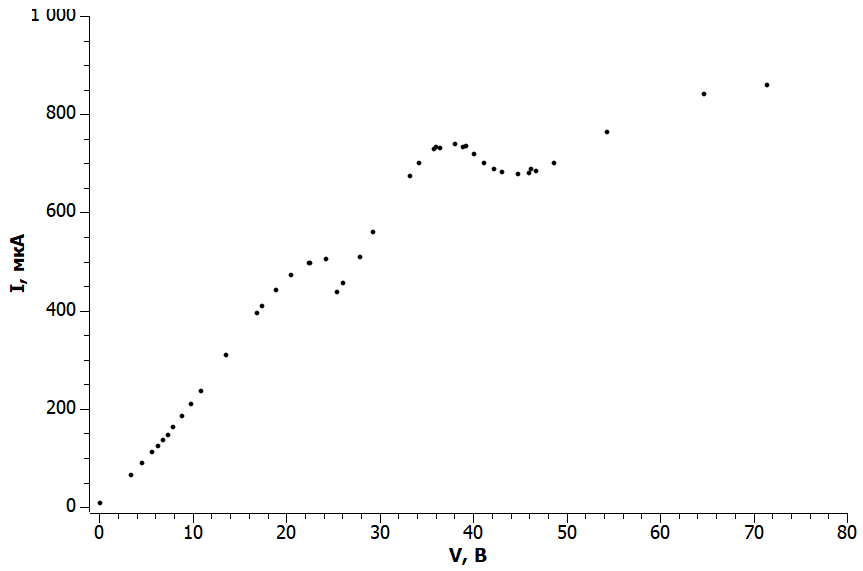
\includegraphics[width=1\linewidth]{images/graph_4.png}
\caption{Вольт-амперная характеристика трёхэлектродной вакуумной лампы при значении запирающего напряжения в 4 В} %% подпись к рисунку
\label{ris:experimoriginal} %% метка рисунка для ссылки на него
\end{minipage}
\hfill 
\begin{minipage}[h]{0.45\linewidth}
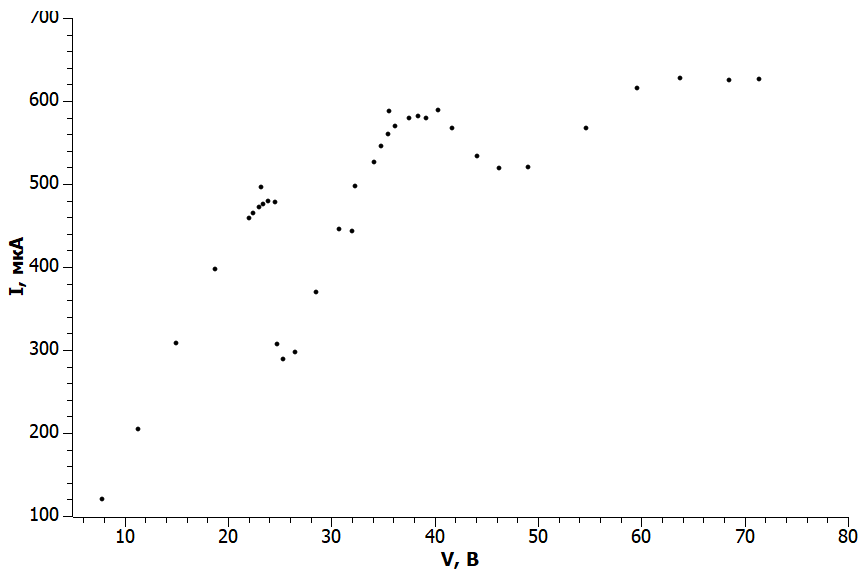
\includegraphics[width=1\linewidth]{images/graph_6.png}
\caption{Вольт-амперная характеристика трёхэлектродной вакуумной лампы при значении запирающего напряжения в 6 В}
\label{ris:experimcoded}
\end{minipage}
\hfill 
\begin{minipage}[h]{0.45\linewidth}
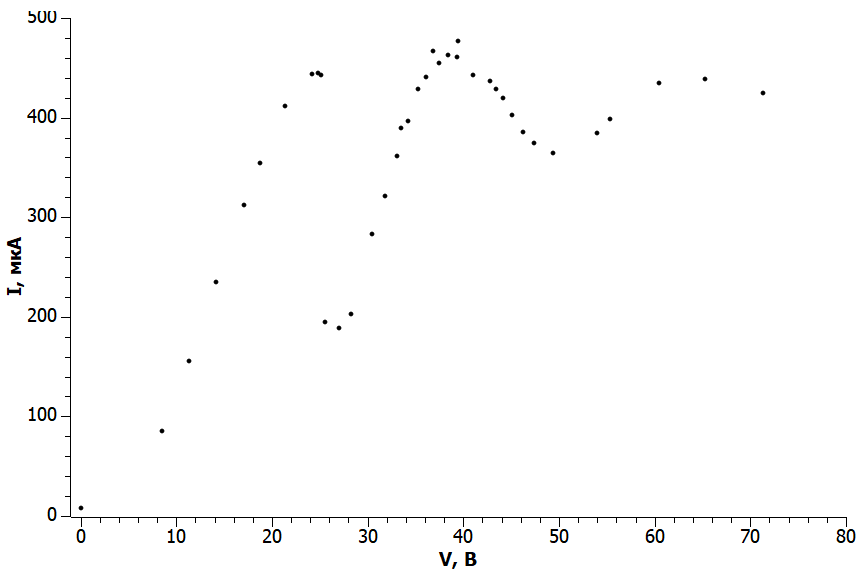
\includegraphics[width=1\linewidth]{images/graph_8.png}
\caption{Вольт-амперная характеристика трёхэлектродной вакуумной лампы при значении запирающего напряжения в 8 В}
\label{ris:experimcoded}
\end{minipage}
\end{center}
\end{figure}

\item Воспользуемся методом из динамического метода и определим энергию первого возбуждения атом гелия. Занесем данные в таблицу 2:

\begin{center}
\begin{tabular}{ |p{3.5cm}||p{1cm}|p{1cm}|p{1cm}|p{1cm}|p{2.5cm}|p{1cm}|p{1cm}|}
 \hline
Задерж. напряжение & $V_{max_1}$ & $V_{max_2}$ & $V_{min_1}$ & $V_{min_2}$ & Погрешность & $\triangle V_{max}$ & $\triangle V_{min}$\\
 \hline
 4 В & 24.2 В & 39.2 В & 25.4 В & 44.8 В & 0.1 В & 15 В & 19.4 В\\
\hline
 6 В & 23.9 В & 38.4 В & 25.3 В & 46.2 В & 0.1 В & 14.5В & 20.9 В\\
\hline
 8 В & 24.8 В & 38.4 В & 27 В & 49.4 В & 0.1 В & 13.6 В & 22.4 В\\
\hline

\end{tabular}
\end{center}

\item Определим значение энергии первого возбуждённого состояния атома гелия. 
\begin{center}
    $\overline{V_{max}} = 14.4$ В \hspace{1cm} $\overline{V_{min}} = 20.9$ В
\end{center}
Погрешности определения средних значений определим, используя формулу
\begin{center}
    $\sigma^2_{V_1} = \sigma^2_{V_4} + \sigma^2_{V_6} + \sigma^2_{V_8}$ - погрешность прибора \\
    $\sigma_{V_2} = \sqrt{\frac{1}{6}\sum (V_i - \overline{V})^2}$ -  погрешность среднего значения \\
    $\sigma_{V_1} = 0.2$ В \hspace{1cm} $\sigma_{V_{max_2}} = 0.4$ В  \hspace{1cm} $\sigma_{V_{min_2}} = 0.9$ В
\end{center}

В итоге получаем:
\begin{center}
    $\overline{V_{max}} = 14.4 \pm 0.5$ В \hspace{1cm} $\overline{V_{min}} = 20.9 \pm 0.9	$ В
\end{center}


Среднее значение первого возбуждённого состояния атома гелия по результатам эксперимента:
\begin{center}
    $V_{exp} = 17.7 \pm 1.1$ эВ (относительная погрешность составляет 6\%)
\end{center}
При этом табличное значение данной величины составляет
\begin{center}
    $V_{th} = 21.6$ эВ
\end{center}

С учётом погрешности, экспериментальные данные немного отличаются от теоретических. Это может быть обусловлено недостаточным количеством измерений в местах максимумови минимумов напряжения. Для решения данной проблемы нужна установка в наш прибор ручки регулировки с более высокой чувствительностью, так как имеющаяся ручка при небольшом повороте уже значительно увеличивает напряжение (порядка 1 Вольта).

\end{enumerate}

\section{Вывод}

В ходе работы был воспроизведён опыт Франка-Герца, подтверждающий наличие дискретных уровней возбуждения атомов. Вольт-амперная характеристика трёхэлектродной вакуумной лампы была измерена двумя способами - динамическим и статическим. По этим ВАХ были экспериментально определены потенциалы возбуждения атомов гелия (одноатомный газ, заполняющий лампу). 
\begin{center}
    $V_{exp_d} = 16.7 \pm 2.5$  эВ \\
    $V_{exp_s} = 17.7 \pm 1.1$ эВ \\
    $V_{th} = 21.6 $ эВ
\end{center}
Видим, что результаты совпадают между собой в пределах погрешности, но немного отличаются от табличного значения. Статический метод оказался более точным, чем динамический. \par
Стоит отметить, что при наличии более совершенной установки можно выполнить более точные измерения ВАХ, тем самым определив потенциалы возбуждения других дискретных уровней, а также потенциалы ионизации.

\end{document}